\documentclass[]{standalone}

\usepackage{adjustbox}

\usepackage{amsmath}

\usepackage{mathrsfs}

\usepackage{circuitikz}
\usepackage{tikz}
\usetikzlibrary{arrows, patterns, decorations.pathmorphing, backgrounds, positioning, fit, petri, shapes, trees, matrix, chains, decorations, decorations.pathreplacing, decorations.fractals, calc,snakes,trees, decorations.markings}

\usepackage{color}
\definecolor{soton}{RGB}{7,51,71}
\colorlet{comms}{red!50!yellow}
\colorlet{payld}{pink!50!purple}
\colorlet{obdh}{green!50!black}

\begin{document}

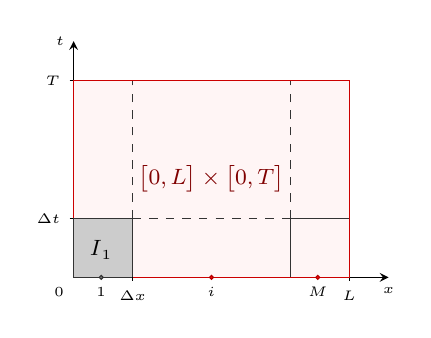
\begin{tikzpicture}

\draw[stealth-] (0,3) node[left] {\tiny{$t$}} -- (0,2.5);
\node[anchor=north east] at (0,0) {\tiny{$0$}};
\draw[-stealth] (3.5, 0) -- (4,0) node[below] {\tiny{$x$}};

\draw[thin] (-0.05, 2.5) node[left] {\tiny{$T$}} -- (0, 2.5);
\draw[thin] (3.5, 0) -- (3.5,-0.05) node[below] {\tiny{$L$}};
\draw[thin, red!80!black, fill=red!4] (0, 2.5) -- (3.5, 2.5) -- (3.5,0) -- (0,0) -- cycle;

\draw[thin] (-0.05, 0.75) node[left] {\tiny{$\Delta t$}} -- (0, 0.75);
\draw[black!80, fill=black!20] (0.75, 0.75) -- (0.75, 0) -- (0,0) -- (0, 0.75) -- cycle;
\draw[thin] (0.75, 0) -- (0.75, -0.05) node[below] {\tiny{$\Delta x$}};

\draw[black!80, fill=black!50] (0.35,0) node[below, black] {\tiny{$1$}} circle (0.025);

\draw[thin, dashed, black!80] (0.75, 0.75) -- (2.75, 0.75);
\draw[thin, black!80] (3.5, 0.75) -- (2.75, 0.75) -- (2.75, 0);
\draw[thin, dashed, black!80] (2.75, 0.75) -- (2.75, 2.5);
\draw[thin, dashed, black!80] (0.75, 0.75) -- (0.75, 2.5);

\draw[red!70!black, fill=red] (3.1,0) node[below, black] {\tiny{$M$}} circle (0.025);
\draw[red!70!black, fill=red] (1.75,0) node[below, black] {\tiny{$i$}} circle (0.025);

\node at (0.35, 0.35) {\footnotesize{$I$}\tiny{$_1$}};
\node[red!50!black] at (1.75, 1.25) {\footnotesize{$\big[0,L\big]\times\big[0,T\big]$}};

\end{tikzpicture}


\end{document}